%%%%%%%%%%%%%%%%%%%%%%%%%%%%%%%%%%%%%%%%%%%%%%%%%%%%%%%%%%%%%%%%%
% MUW Presentation
% LaTeX Template
% Version 1.0 (27/12/2016)
%
% License:
% CC BY-NC-SA 4.0 (http://creativecommons.org/licenses/by-nc-sa/3.0/)
%
% Created by:
% Nicolas Ballarini, CeMSIIS, Medical University of Vienna
% nicoballarini@gmail.com
% http://statistics.msi.meduniwien.ac.at/
%
% Customized for UAH by:
% David F. Barrero, Departamento de Automática, UAH
%%%%%%%%%%%%%%%%%%%%%%%%%%%%%%%%%%%%%%%%%%%%%%%%%%%%%%%%%%%%%%%%%

\documentclass[10pt,compress]{beamer} % Change 10pt to make fonts of a different size
\mode<presentation>

\usepackage[spanish]{babel}
\usepackage{fontspec}
\usepackage{tikz}
\usepackage{etoolbox}
\usepackage{xcolor}
\usepackage{xstring}
\usepackage{listings}

\usetheme{UAH}
\usecolortheme{UAH}
\setbeamertemplate{navigation symbols}{}
\setbeamertemplate{caption}[numbered]

%%%%%%%%%%%%%%%%%%%%%%%%%%%%%%%%%%%%%%%%%%%%%%%%%%%%%%%%%%%%%%%%%
%% Presentation Info
\title[Using Git]{\IfStrEq{\modo}{VIDEOJUEGOS}{Using Git and GitHub}{Short Introduction to SCM and Git}}
\author{\IfStrEq{\modo}{VIDEOJUEGOS}{\asignatura}{D. Rodríguez, D. F. Barrero}}
\institute{\IfStrEq{\modo}{VIDEOJUEGOS}{}{University of Alcalá}}
\date{}
%%%%%%%%%%%%%%%%%%%%%%%%%%%%%%%%%%%%%%%%%%%%%%%%%%%%%%%%%%%%%%%%%


%%%%%%%%%%%%%%%%%%%%%%%%%%%%%%%%%%%%%%%%%%%%%%%%%%%%%%%%%%%%%%%%%
%% Descomentar para habilitar barra de navegación superior
\setNavigation
%%%%%%%%%%%%%%%%%%%%%%%%%%%%%%%%%%%%%%%%%%%%%%%%%%%%%%%%%%%%%%%%%

%%%%%%%%%%%%%%%%%%%%%%%%%%%%%%%%%%%%%%%%%%%%%%%%%%%%%%%%%%%%%%%%%
%% Configuración de logotipos en portada
%% Opacidad de los logotipos
\newcommand{\opacidad}{1}
%% Descomentar para habilitar logotipo en pié de página de portada
\renewcommand{\logoUno}{Images/isg.png}
%% Descomentar para habilitar logotipo en pié de página de portada
%\renewcommand{\logoDos}{Images/CCLogo.png}
%% Descomentar para habilitar logotipo en pié de página de portada
%\renewcommand{\logoTres}{Images/ALogo.png}
%% Descomentar para habilitar logotipo en pié de página de portada
%\renewcommand{\logoCuatro}{Images/ELogo.png}
%%%%%%%%%%%%%%%%%%%%%%%%%%%%%%%%%%%%%%%%%%%%%%%%%%%%%%%%%%%%%%%%%

%%%%%%%%%%%%%%%%%%%%%%%%%%%%%%%%%%%%%%%%%%%%%%%%%%%%%%%%%%%%%%%%%
%% FOOTLINE
%% Comment/Uncomment the following blocks to modify the footline
%% content in the body slides.


%% Option A: Title and institute
\footlineA
%% Option B: Author and institute
%\footlineB
%% Option C: Title, Author and institute
%\footlineC
%%%%%%%%%%%%%%%%%%%%%%%%%%%%%%%%%%%%%%%%%%%%%%%%%%%%%%%%%%%%%%%%%

\begin{document}

%%%%%%%%%%%%%%%%%%%%%%%%%%%%%%%%%%%%%%%%%%%%%%%%%%%%%%%%%%%%%%%%%
% Use this block for a blue title slide with modified footline
{\titlepageBlue
    \begin{frame}
        \titlepage
    \end{frame}
}

\begin{frame}[plain]{}
   \begin{block}{Objectives}
      \begin{enumerate}
         \item Understand the need of SCM
         \item Implement software development workflows with Git and Github
      \end{enumerate}
   \end{block}

   \begin{block}{Bibliography}
      \begin{enumerate}
          \item GitHub Guides. \href{https://guides.github.com/}{(Link)}
      \end{enumerate} 
   \end{block}
\end{frame}

{
\disableNavigation{white}
\begin{frame}[shrink]{Table of Contents}
 \frametitle{Table of Contents}
 \tableofcontents
  % You might wish to add the option [pausesections]
\end{frame}
}


\section{Version control}

%%%%%%%%%%%%%%%%%%%%%%%%%%%%%%%%%%%%%%%%%%%%%%%%%%%%%%%%%%%%%%%%%%%%%%

\begin{frame}{Version control}

\begin{block}{Version control systems}
Version control systems (VCS) keep track of changes to source code.
Allows multiple people to edit a project in a predictable manner.
\end{block}

Main open source VCS 
\begin{itemize}
 \item 1982 RCS
 \item 1990 CVS
 \item 2000 Subversion
 \item 2005 Git/Mercurial
\end{itemize}

There are many proprietary ones but \texttt{Git} is now the most popular one by far.

All software should be under a version control system, if not, it ain't software!

\end{frame}


%%%%%%%%%%%%%%%%%%%%%%%%%%%%%%%%%%%%%%%%%%%%%%%%%%%%%%%%%%%%%%%%%%%%%%
\section{Git}

%%%%%%%%%%%%%%%%%%%%%%%%%%%%%%%%%%%%%%%%%%%%%%%%%%%%%%%%%%%%%%%%%%%%%%
\subsection{What is Git?}

%%%%%%%%%%%%%%%%%%%%%%%%%%%%%%%%%%%%%%%%%%%%%%%%%%%%%%%%%%%%%%%%%%%%%%
\begin{frame}{Git}{What is Git?}

\centering 
\includegraphics[width=.2\textwidth]{figs/Git-Logo-2Color.eps}

\begin{columns}
\column{.70\textwidth}
Git is an open source distributed version control system, created by Linus Torvald.

\url{https://git-scm.com/}
\\
\href{https://try.github.io/levels/1/challenges/1}{(Interactive tutorial)}


\column{.30\textwidth}
\begin{center}
 \includegraphics[width=.8\textwidth]{figs/torvalds-to-nvidia}
\end{center}
\end{columns}

\end{frame}

%%%%%%%%%%%%%%%%%%%%%%%%%%%%%%%%%%%%%%%%%%%%%%%%%%%%%%%%%%%%%%%%%%%%%%
\subsection{Git sites}
\begin{frame}{Git}{Git sites}


It is easier to start with free hosting sites instead of maintaining your own server.

\begin{itemize}
\item \alert{GitHub}: public repositories (as many as you want), but private ones are not free (except for academia). It is now part of Microsoft
 \item \alert{Bitbucket}: allow us to keep private repositories limiting the number of collaborators.
 \item \alert{GitLab}: both public and private without limitations. It is becoming more popular.
 \item Others ...
\end{itemize}

It is typically used as central repository:
\begin{itemize}
 \item from which everyone pulls other people’s changes
 \item to which everyone pushes changes they have made
\end{itemize}

\end{frame}

%%%%%%%%%%%%%%%%%%%%%%%%%%%%%%%%%%%%%%%%%%%%%%%%%%%%%%%%%%%%%%%%%%%%%
\subsection{Git vs. SVN}

%%%%%%%%%%%%%%%%%%%%%%%%%%%%%%%%%%%%%%%%%%%%%%%%%%%%%%%%%%%%%%%%%%%%%
\begin{frame}{Git}{Git vs. SVN (I)}
\begin{center}
\begin{columns}
	\column{.50\linewidth}
	\centering Centralized (SVN)\\\smallskip
\includegraphics[width=\linewidth]{figs/centralized.png}
	\column{.50\linewidth}
	\centering Distributed (Git)\\\smallskip
\includegraphics[width=\linewidth]{figs/distributed.png}
\end{columns}

\tiny \href{http://softwareengineering.stackexchange.com/questions/35074/im-a-subversion-geek-why-should-i-consider-or-not-consider-mercurial-or-git-or}{(Source)}
\end{center}
	Disclaimer: Do not pay attention to the labels of these diagrams
\end{frame}

%%%%%%%%%%%%%%%%%%%%%%%%%%%%%%%%%%%%%%%%%%%%%%%%%%%%%%%%%%%%%%%%%%%%%


\begin{frame}{Git}{Git vs. SVN (II)}
\begin{center}
\begin{columns}
	\column{.50\linewidth}
	\centering Fully distributed (Git)\\\smallskip
	\includegraphics[width=\linewidth]{figs/fulldistributed.png}
	\tiny \href{http://softwareengineering.stackexchange.com/questions/35074/im-a-subversion-geek-why-should-i-consider-or-not-consider-mercurial-or-git-or}{(Source)}

	\column{.50\linewidth}
	\begin{block}{Key Git concepts to know}
	\begin{itemize}
	\item \texttt{repository} (local or not)
	\item \texttt{clone}
	\item \texttt{commit}, \texttt{push}
	\item \texttt{pull}, \texttt{fetch} 
	\item \texttt{remote}, \texttt{origin}
	\item \texttt{merge}
	\end{itemize}
	\end{block}
\end{columns}
\end{center}
\end{frame}


%%%%%%%%%%%%%%%%%%%%%%%%%%%%%%%%%%%%%%%%%%%%%%%%%%%%%%%%%%%%%%%%%%%%%%
\section{Using Git}

%%%%%%%%%%%%%%%%%%%%%%%%%%%%%%%%%%%%%%%%%%%%%%%%%%%%%%%%%%%%%%%%%%%%%%
%\subsection{Repository initialization and clonning}

%%%%%%%%%%%%%%%%%%%%%%%%%%%%%%%%%%%%%%%%%%%%%%%%%%%%%%%%%%%%%%%%%%%%%%

%\begin{frame}[fragile]{Using Git}{Basic commands: Repository initialization}

%When using Git for the first time:

%\begin{verbatim}
%git config --global user.email user@uah.es
%git config --global user.name  "Jane Doe"
%\end{verbatim}

%Initialization:

%\begin{verbatim}
%mkdir /path/to/your/project
%cd /path/to/your/project
%git init
%git remote add origin https://<where>/<path>/<project.git>
%git push -u origin --all # pushes up the repo and its refs for the first time
%\end{verbatim}

%\end{frame}

%%%%%%%%%%%%%%%%%%%%%%%%%%%%%%%%%%%%%%%%%%%%%%%%%%%%%%%%%%%%%%%%%%%%%%
%\begin{frame}{Using Git}{Basic commands: Repository clonning}

%To work with someone else’s repository, we first need to \emph{clone} it to get a
%local copy.

%\texttt{git clone <repo>}

%E.g.:

%\texttt{git clone https://github.com/danrodgar/gitSlides.git}

%\begin{footnotesize}Note: once cloned, you can edit the repository as much as you want. No changes make their way back to the ‘central’ repository until you explicitly do so.
%\end{footnotesize}
%\end{frame}


%%%%%%%%%%%%%%%%%%%%%%%%%%%%%%%%%%%%%%%%%%%%%%%%%%%%%%%%%%%%%%%%%%%%%%
%\subsection{Basic commands}


%\begin{frame}[fragile]{Using Git}{Basic commands: tracking files}

%Then, we can start tracking files. To do so, we need to \texttt{add}, \texttt{commit}, and \texttt{push} the file(s) that we want to track.

%\begin{verbatim}
%echo "A new file..." >> Readme.md
%git add Readme.md
%git commit -m 'Initial commit'
%git push -u origin master
%\end{verbatim}

%\end{frame}


%%%%%%%%%%%%%%%%%%%%%%%%%%%%%%%%%%%%%%%%%%%%%%%%%%%%%%%%%%%%%%%%%%%%%%
%%\begin{frame}{Using Git}{Basic commands: Pulling}

% \begin{columns}
% 	\column{.50\linewidth}
% 	\centering Centralized (SVN)\\\smallskip
% \includegraphics[width=\linewidth]{figs/centralized.png}
% 	\column{.50\linewidth}
% 	\centering Distributed (Git)\\\smallskip
% \includegraphics[width=\linewidth]{figs/distributed.png}
% \end{columns}
% To integrate all changes other people have made since you
% cloned/pulled: \texttt{git pull}

%%\begin{itemize}
%% \item If you have made local changes you have to \\
%% \texttt{git stash} \\
%% before pulling, then \\
%% \texttt{git stash pop} \\
%% afterwards

%% \item You can see which files you've modified with\\
%%  \texttt{git status}

%% \item You can permanently remove your local changes by \\
%% \texttt{git checkout <file>}
%%\end{itemize}

%%\end{frame}


%%%%%%%%%%%%%%%%%%%%%%%%%%%%%%%%%%%%%%%%%%%%%%%%%%%%%%%%%%%%%%%%%%%%%%
%\begin{frame}{Using Git}{Basic commands: Pushing}

%\texttt{git add <file>} makes git track the file <file>

%Or to record all changes into a commit (notice the ‘.’):

%\texttt{git commit .}

%\texttt{git push origin master} This pushes all new commits to the repository.


%\end{frame}


%%%%%%%%%%%%%%%%%%%%%%%%%%%%%%%%%%%%%%%%%%%%%%%%%%%%%%%%%%%%%%%%%%%%%%
\subsection{Conflicts}
\begin{frame}{Using Git}{Conflicts}

If two people both modify the same file, the first to push \emph{wins}.
The second person will have to pull and merge before pushing.

\begin{itemize}
	\item Changes in different parts of a file are automatically merged
	\item Changes in the same part of a file cause conflicts
	\begin{itemize}
		\item Select either your changes or remote, or a mix of the two
	\end{itemize}
%\item Two merging cases: have / haven't committed
\end{itemize}
\end{frame}

%%%%%%%%%%%%%%%%%%%%%%%%%%%%%%%%%%%%%%%%%%%%%%%%%%%%%%%%%%%%%%%%%%%%%%
%\begin{frame}{Using Git}{Merge and conflicts: \texttt{diff}}

%\texttt{diff -u <old file> <new file>}

%This command shows what changes you would need to apply to old file to change it into
%new file.

%Lines beginning with:
%\begin{itemize}
% \item \texttt{- - -} or \texttt{+++} tell you the old / new filenames
% \item \texttt{@@} points to where within the file you are looking \\
%       (i.e. a space) are lines that are unchanged
% \item \texttt{-} is a deleted line
% \item \texttt{+} is a newly added line
%\end{itemize}

%\end{frame}

%%%%%%%%%%%%%%%%%%%%%%%%%%%%%%%%%%%%%%%%%%%%%%%%%%%%%%%%%%%%%%%%%%%%%%
%\begin{frame}[fragile]{Using Git}{Merge and conflicts: \texttt{diff} example}

%\begin{scriptsize}
%\begin{columns}
%	\column{.50\linewidth}
%	  \begin{verbatim}
%#include <stdio.h>
%int main() {
%    printf("Hello World\n");
%}
%\end{verbatim}
%	\column{.50\linewidth}
%\begin{verbatim}
%#include <stdio.h>
%int main(int argc, char *argv[]) {
%  printf("Hello World\n");
%  return 0;
%}
%\end{verbatim}
%\end{columns}

%Applying the \texttt{diff} command:
%\begin{verbatim}
%$ diff -u hello.c hello_new.c > hello.patch
%\end{verbatim}

%We get the following patch:
%\begin{verbatim}
%--- hello.c	2014-10-07 18:17:49.000000000 +0530
%+++ hello_new.c	2014-10-07 18:17:54.000000000 +0530
%@@ -1,5 +1,6 @@
% #include <stdio.h>
%-int main() {
%+int main(int argc, char *argv[]) {
% 	printf("Hello World\n");
%+	return 0;
% }
%\end{verbatim}
%\end{scriptsize}


%\end{frame}

%%%%%%%%%%%%%%%%%%%%%%%%%%%%%%%%%%%%%%%%%%%%%%%%%%%%%%%%%%%%%%%%%%%%%%

%\begin{frame}{Using Git}{Merge and conflicts: Applying \texttt{diff} changes (patch command)}

%After the \texttt{patch.diff} is created as:

%\texttt{diff -u <old file> <new file> > file.patch }

%We can apply it with the \texttt{patch} command:

%\texttt{patch < file.patch}

%Note that the \texttt{file.patch} knows the name of the file to be patched.


%\end{frame}

%%%%%%%%%%%%%%%%%%%%%%%%%%%%%%%%%%%%%%%%%%%%%%%%%%%%%%%%%%%%%%%%%%%%%%

%\begin{frame}{Using Git}{Merge and conflicts: Original Patch!}

%\centering
%\includegraphics[width=.4\textwidth,height=\textheight,keepaspectratio]{figs/patch.png}

%\end{frame}


%%%%%%%%%%%%%%%%%%%%%%%%%%%%%%%%%%%%%%%%%%%%%%%%%%%%%%%%%%%%%%%%%%%%%%
\subsection{Commits}
\begin{frame}{Using Git}{Commits}

\begin{itemize}
% \item Merge commits record where parallel development unified
% \item How does Git keep track of things when parallel development
%happens?
\item Every commit has an ID (its hash)
%	, which is a 40 character SHA-1
%hash based on the commit's content. Not guaranteed to be
%unique; but it probably is
\end{itemize}

\end{frame}

%%%%%%%%%%%%%%%%%%%%%%%%%%%%%%%%%%%%%%%%%%%%%%%%%%%%%%%%%%%%%%%%%%%%%%
\subsection{Branches}
\begin{frame}{Using Git}{Branches}

\centering \includegraphics[width=.8\textwidth]{figs/branching}

\flushleft Branches are used extensively (e.g. some like feature branches).

\begin{itemize}
 \item A repository (local and remote) can have explicit branches
 \item The default branch is called \alert{master}
 %		\texttt{git branch <name>} creates branches\\
 % 		\texttt{git checkout <branch name>} switch branches\\
 \item A \alert{merge} is a fusion between two branches
%(i.e. you say “I want to merge another branch into me”)
\end{itemize}

Do no use branches in the project!

\end{frame}

\subsection{Tags}
\begin{frame}{Using Git}{Tags}

A tag is a pointer to a specific point in the repository history
\begin{itemize}
	\item Tags usually have names (e.g. ``v1.1'')
 \item Widely used to keep and publish software releases
\end{itemize}

You might try to tag your project

\end{frame}



%%%%%%%%%%%%%%%%%%%%%%%%%%%%%%%%%%%%%%%%%%%%%%%%%%%%%%%%%%%%%%%%%%%%%%
% \subsection{Tags}
% \begin{frame}{Using Git}{Tags}
% 	TODO
% \end{frame}

%%%%%%%%%%%%%%%%%%%%%%%%%%%%%%%%%%%%%%%%%%%%%%%%%%%%%%%%%%%%%%%%%%%%%%
%\subsection{Advanced Git}
%\begin{frame}{Using Git}{Advanced Git: Getting an old commit}

%Sometimes you need to get an old file or discard some changes. With

%\begin{itemize}
% \item \texttt{git log}
% \item \texttt{git log -- oneline}
%\end{itemize}

%we can check previous commits and select one with \texttt{checkout}, e.g.:
%\begin{itemize}
% \item \texttt{git checkout c71d008}
%\end{itemize}

%\end{frame}


%%%%%%%%%%%%%%%%%%%%%%%%%%%%%%%%%%%%%%%%%%%%%%%%%%%%%%%%%%%%%%%%%%%%%%
\subsection{Good practices}
\begin{frame}{Using Git}{Good practices}

%Tipically changes are checked by someone other than their
%author before being merged into master. This kind of \textbf{code review} is is naturally captured by pull requests in Git.

Learn on the job: the best way to learn it is by using it. 

\bigskip

Best practices
\begin{itemize}
  \item Regularly push and pull (at least daily, in general)
  \item Don't push half-baked changes 
  \item Don't pull if you're in the middle of a task
  \item Never commit temporal/intermediate files
  \item The master must be a clean and functional version of the project
\end{itemize}

\end{frame}

%%%%%%%%%%%%%%%%%%%%%%%%%%%%%%%%%%%%%%%%%%%%%%%%%%%%%%%%%%%%%%%%%%%%%%

\section{GitHub}
\subsection{Features}
\begin{frame}{GitHub}{Features}
	\begin{columns}
	\column{.10\textwidth}
	\column{.50\textwidth}
		Free Git hosting provider
		\begin{itemize}
			\item Free public repositories
		\end{itemize}
		User interface to Git
		\begin{itemize}
			\item Repository browser
		\end{itemize}
		Added value Git operations
		\begin{itemize}
			\item Social network
			\item Collaborative tools
			\item Pull requests	
			\item Issue tracking
			\item Web hosting
			\item Markdown integration
			\item Organizations
		\end{itemize}
	\column{.30\textwidth}
	\begin{center}
 		\includegraphics[width=.8\textwidth]{figs/github-logo}
	\end{center}
	\column{.10\textwidth}
	\end{columns}
\end{frame}

\begin{frame}{GitHub}{Key concepts}
	\begin{block}{Key GitHub concepts to know}
	\begin{itemize}
	\item \texttt{Pull request}
	\item \texttt{Fork}
	\end{itemize}
	\end{block}
\end{frame}

\subsection{README}
\begin{frame}{GitHub}{README}
	Special file: README.md
	\begin{itemize}
		\item Contains information about the project
		\item Automatically visualized
		\item md means Markdown
	\end{itemize}
\end{frame}

\subsection{Markdown}
\begin{frame}[fragile]{Markdown (I)}
 	\centering 
\includegraphics[width=0.3\textwidth]{figs/logo-md.png}
	\bigskip

	\begin{columns}
	\column{.5\textwidth}
	Markdown: Trivial markup
	\begin{itemize}
		\item Simple
		\item Very simple
		\item Extremely simple
		\item Did I say it's simple?
	\end{itemize}

	\column{.5\textwidth}
	VERY powerful
	\begin{itemize}
		\item Several outputs
		\item Professional quality
		\item ... and simple!
	\end{itemize}
	\end{columns}


\end{frame}

\begin{frame}[fragile]{Markdown (II)}
	\vspace{-0.3cm}
	\begin{columns}
	\column{.6\textwidth}
		\begin{exampleblock}{Markdown example}
			\vspace{-0.3cm}
			\begin{lstlisting}[mathescape]
# I am a header
## I am a subheader

Regular, *italic* and **bold**

- List item 1
- List item 2

[I am a link](http://foo.com)

![I am a pic](markdown.png)

~~~C
printf("Hello, world");
~~~
\end{lstlisting}
			\vspace{-0.2cm}
		\end{exampleblock}
	\column{.4\textwidth}
 		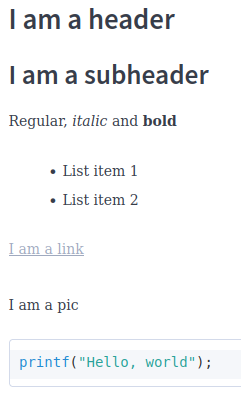
\includegraphics[width=0.6\textwidth]{figs/md.png}
	\end{columns}
\end{frame}



%\subsection{GitHub Pages}

%\begin{frame}{GitHub}{GitHub Pages}
%	Pages integrate web site in the GitHub workflow
%	\begin{itemize}
%		\item Creation of full web sites
%		\item Project web site
%		\item Documentation
%		\item Based on Markdown (and something named \textit{Jekyll}
%	\end{itemize}

%	GitHub locates the content to publish in three places:
%	\begin{itemize}
%		\item A branch named \texttt{gh-pages}
%		\item master itself
%		\item A folder \texttt{docs} in master
%		\item \textbf{Page available on \url{https://<username>.github.io/<repository>}}
%	\end{itemize}

%	By default, Pages are disabled 
%	\begin{itemize}
%		\item Enable them in settings
%	\end{itemize}

%	User Page. Site accesible in \url{https://<username>.github.io}
%	\begin{itemize}
%		\item The repository must be named \texttt{<username>.github.io}
%		\item master branch
%	\end{itemize}
%\end{frame}

% %%%%%%%%%%%%%%%%%%%%%%%%%%%%%%%%%%%%%%%%%%%%%%%%%%%%%%%%%%%%%%%%%%%%%%
% \begin{frame}{}
%
% \end{frame}
%


%%%%%%%%%%%%%%%%%%%%%%%%%%%%%%%%%%%%%%%%%%%%%%%%%%%%%%%%%%%%%%%%%%%%%%


\end{document}
